% Options for packages loaded elsewhere
\PassOptionsToPackage{unicode}{hyperref}
\PassOptionsToPackage{hyphens}{url}
%
\documentclass[
  12pt,
]{article}
\usepackage{amsmath,amssymb}
\usepackage{iftex}
\ifPDFTeX
  \usepackage[T1]{fontenc}
  \usepackage[utf8]{inputenc}
  \usepackage{textcomp} % provide euro and other symbols
\else % if luatex or xetex
  \usepackage{unicode-math} % this also loads fontspec
  \defaultfontfeatures{Scale=MatchLowercase}
  \defaultfontfeatures[\rmfamily]{Ligatures=TeX,Scale=1}
\fi
\usepackage{lmodern}
\ifPDFTeX\else
  % xetex/luatex font selection
\fi
% Use upquote if available, for straight quotes in verbatim environments
\IfFileExists{upquote.sty}{\usepackage{upquote}}{}
\IfFileExists{microtype.sty}{% use microtype if available
  \usepackage[]{microtype}
  \UseMicrotypeSet[protrusion]{basicmath} % disable protrusion for tt fonts
}{}
\makeatletter
\@ifundefined{KOMAClassName}{% if non-KOMA class
  \IfFileExists{parskip.sty}{%
    \usepackage{parskip}
  }{% else
    \setlength{\parindent}{0pt}
    \setlength{\parskip}{6pt plus 2pt minus 1pt}}
}{% if KOMA class
  \KOMAoptions{parskip=half}}
\makeatother
\usepackage{xcolor}
\usepackage[margin=1in]{geometry}
\usepackage{longtable,booktabs,array}
\usepackage{calc} % for calculating minipage widths
% Correct order of tables after \paragraph or \subparagraph
\usepackage{etoolbox}
\makeatletter
\patchcmd\longtable{\par}{\if@noskipsec\mbox{}\fi\par}{}{}
\makeatother
% Allow footnotes in longtable head/foot
\IfFileExists{footnotehyper.sty}{\usepackage{footnotehyper}}{\usepackage{footnote}}
\makesavenoteenv{longtable}
\usepackage{graphicx}
\makeatletter
\def\maxwidth{\ifdim\Gin@nat@width>\linewidth\linewidth\else\Gin@nat@width\fi}
\def\maxheight{\ifdim\Gin@nat@height>\textheight\textheight\else\Gin@nat@height\fi}
\makeatother
% Scale images if necessary, so that they will not overflow the page
% margins by default, and it is still possible to overwrite the defaults
% using explicit options in \includegraphics[width, height, ...]{}
\setkeys{Gin}{width=\maxwidth,height=\maxheight,keepaspectratio}
% Set default figure placement to htbp
\makeatletter
\def\fps@figure{htbp}
\makeatother
\setlength{\emergencystretch}{3em} % prevent overfull lines
\providecommand{\tightlist}{%
  \setlength{\itemsep}{0pt}\setlength{\parskip}{0pt}}
\setcounter{secnumdepth}{-\maxdimen} % remove section numbering
\newlength{\cslhangindent}
\setlength{\cslhangindent}{1.5em}
\newlength{\csllabelwidth}
\setlength{\csllabelwidth}{3em}
\newlength{\cslentryspacingunit} % times entry-spacing
\setlength{\cslentryspacingunit}{\parskip}
\newenvironment{CSLReferences}[2] % #1 hanging-ident, #2 entry spacing
 {% don't indent paragraphs
  \setlength{\parindent}{0pt}
  % turn on hanging indent if param 1 is 1
  \ifodd #1
  \let\oldpar\par
  \def\par{\hangindent=\cslhangindent\oldpar}
  \fi
  % set entry spacing
  \setlength{\parskip}{#2\cslentryspacingunit}
 }%
 {}
\usepackage{calc}
\newcommand{\CSLBlock}[1]{#1\hfill\break}
\newcommand{\CSLLeftMargin}[1]{\parbox[t]{\csllabelwidth}{#1}}
\newcommand{\CSLRightInline}[1]{\parbox[t]{\linewidth - \csllabelwidth}{#1}\break}
\newcommand{\CSLIndent}[1]{\hspace{\cslhangindent}#1}
\newenvironment{cols}[1][]{}{}

\newenvironment{col}[1]{\begin{minipage}{#1}\ignorespaces}{%
\end{minipage}
\ifhmode\unskip\fi
\aftergroup\useignorespacesandallpars}

\def\useignorespacesandallpars#1\ignorespaces\fi{%
#1\fi\ignorespacesandallpars}

\makeatletter
\def\ignorespacesandallpars{%
  \@ifnextchar\par
    {\expandafter\ignorespacesandallpars\@gobble}%
    {}%
}
\makeatother
\renewcommand{\and}{\\}
\usepackage{float}
\floatplacement{figure}{H}
\usepackage{booktabs}
\usepackage{longtable}
\usepackage{array}
\usepackage{multirow}
\usepackage{wrapfig}
\usepackage{float}
\usepackage{colortbl}
\usepackage{pdflscape}
\usepackage{tabu}
\usepackage{threeparttable}
\usepackage{threeparttablex}
\usepackage[normalem]{ulem}
\usepackage{makecell}
\usepackage{xcolor}
\ifLuaTeX
  \usepackage{selnolig}  % disable illegal ligatures
\fi
\IfFileExists{bookmark.sty}{\usepackage{bookmark}}{\usepackage{hyperref}}
\IfFileExists{xurl.sty}{\usepackage{xurl}}{} % add URL line breaks if available
\urlstyle{same}
\hypersetup{
  pdfauthor={Teng Li(7373086); Shiya Gao(300381032); Chuhan Yue(300376046); Yang Lyu(8701121)},
  hidelinks,
  pdfcreator={LaTeX via pandoc}}

\title{\vspace{-4em}MAT5314 Project 1: Data Visualization}
\author{Teng Li(7373086) \and Shiya Gao(300381032) \and Chuhan
Yue(300376046) \and Yang Lyu(8701121)}
\date{}

\begin{document}
\maketitle

\hypertarget{introduction}{%
\section{Introduction}\label{introduction}}

A data set of the 2016 US election polls was given. In this project we
aim to understand the data structure by creating various visualizations.

First, we would like to give a brief introduction to the U.S. election
system as it is crucial to understand the background of the data. Voters
in each state vote to choose the President of the United States. The
candidate who wins the majority of the votes will receive all the
electoral votes in that state. Then the sum of the electoral votes in
each state is calculated. The total number of electoral votes is 538.
The candidate who wins half of the votes plus 1 will win and become the
new President of the United States. Since each state has a different
number of electoral votes, it is crucial for electors to win in several
key states. The reason is that if a candidate wins a certain state, he
will win all the electoral votes in that state. Texas, for example,
counts for 38 electoral votes during the election, it is therefore a
tight competition in states with more votes.

Analysis on poll result can be very difficult due to the fact that
carrying out a public opinion poll is generally difficult. The
experimental design plays a profound rule in these surveys, as sometimes
it is hard to achieve an unbiased sample. On the other hand, one might
not be able to obtain the final result that can be compared with the
poll result. Finally it can be very expensive to carry out a qualitative
poll under budget constrains. However, election poll result is a
desirable measurement we can study. Large institutions design the survey
and gather public opinions. Moreover, we immediately know with high
accuracy and details on who wins the election at the end. It is
therefore worthy to analyze the poll results and make some inferences,
perhaps even compare results between each election. Thus, we want to
analyze some of the key factors given by our poll result data and
compare with the actual election result for the candidate's victory.

\hypertarget{method}{%
\section{Method}\label{method}}

The data set was published by FiveThirtyEight to illustrate the
reliability and quality of each pollster to which a letter grade ranging
from A+ to D- was given. We first analyzed key individual variables in
the data, then we sought to draw conclusions on the relationship between
some of the key variables. To achieve this, we use various R packages to
present the data set and to plot the graphs.

\hypertarget{section-1-data-dictionary}{%
\section{Section 1: Data Dictionary}\label{section-1-data-dictionary}}

We first created a data variable definition table to give an initial
understanding of the data. We formed the table by collecting each
variable from the data, listed in the Variables column. We then looked
at the size and the data type of each variable to understand its nature.
An example consisting of a few variable values was given to illustrate
what the variable might look like. We then calculated the number of
unique and missing values in each variable. As one can see, there were a
few variables with high percentage of missing values, for which we have
discussed further in details in the subsequent sections. Finally, we
gave a comment for each variable to briefly explains what it means and
what it represents. The data dictionary is listed in Table 1:

\begin{table}[!h]

\caption{\label{tab:unnamed-chunk-3}Data Variable Definition}
\centering
\resizebox{\linewidth}{!}{
\fontsize{10}{12}\selectfont
\begin{tabular}[t]{lrl>{\raggedright\arraybackslash}p{8em}rrl}
\toprule
\textbf{Variables} & \textbf{Size} & \textbf{Type} & \textbf{Example} & \textbf{Number.Unique} & \textbf{Number.Missing} & \textbf{Comment}\\
\midrule
\cellcolor{gray!6}{state} & \cellcolor{gray!6}{4208} & \cellcolor{gray!6}{character} & \cellcolor{gray!6}{U.S., New Mexico, Virginia} & \cellcolor{gray!6}{57} & \cellcolor{gray!6}{0} & \cellcolor{gray!6}{The name of the state (or national) where the election is held}\\
startdate & 4208 & character & 2016/11/3, 2016/11/1, 2016/11/2 & 352 & 0 & Start date of poll\\
\cellcolor{gray!6}{enddate} & \cellcolor{gray!6}{4208} & \cellcolor{gray!6}{character} & \cellcolor{gray!6}{2016/11/6, 2016/11/7, 2016/11/5} & \cellcolor{gray!6}{345} & \cellcolor{gray!6}{0} & \cellcolor{gray!6}{End date of poll}\\
pollster & 4208 & character & ABC News/Washington Post, Google Consumer Surveys, Ipsos & 196 & 0 & Organization name that conducts or analyzes opinion polls\\
\cellcolor{gray!6}{grade} & \cellcolor{gray!6}{4208} & \cellcolor{gray!6}{character} & \cellcolor{gray!6}{A+, B, A-} & \cellcolor{gray!6}{11} & \cellcolor{gray!6}{429} & \cellcolor{gray!6}{Grade assigned by Fivethirtyeight to pollster}\\
\addlinespace
samplesize & 4208 & integer & 2220, 26574, 2195 & 1767 & 1 & Sample size of polls for each pollster\\
\cellcolor{gray!6}{population} & \cellcolor{gray!6}{4208} & \cellcolor{gray!6}{character} & \cellcolor{gray!6}{lv, rv, a} & \cellcolor{gray!6}{4} & \cellcolor{gray!6}{0} & \cellcolor{gray!6}{Type of population being polled}\\
rawpoll\_clinton & 4208 & numeric & 47, 38.03, 42 & 1312 & 0 & Poll Percentage for Hillary Clinton\\
\cellcolor{gray!6}{rawpoll\_trump} & \cellcolor{gray!6}{4208} & \cellcolor{gray!6}{numeric} & \cellcolor{gray!6}{43, 35.69, 39} & \cellcolor{gray!6}{1385} & \cellcolor{gray!6}{0} & \cellcolor{gray!6}{Poll Percentage for Donald Trump}\\
rawpoll\_johnson & 4208 & numeric & 4, 5.46, 6 & 585 & 1409 & Poll Percentage for Gary Johnson\\
\addlinespace
\cellcolor{gray!6}{rawpoll\_mcmullin} & \cellcolor{gray!6}{4208} & \cellcolor{gray!6}{numeric} & \cellcolor{gray!6}{NA, 24, 27.6} & \cellcolor{gray!6}{17} & \cellcolor{gray!6}{4178} & \cellcolor{gray!6}{Poll Percentage for Evan Mcmullin}\\
adjpoll\_clinton & 4208 & numeric & 45.20163, 43.34557, 42.02638 & 4200 & 0 & Adjusted percentage for Hillary Clinton\\
\cellcolor{gray!6}{adjpoll\_trump} & \cellcolor{gray!6}{4208} & \cellcolor{gray!6}{numeric} & \cellcolor{gray!6}{41.7243, 41.21439, 38.8162} & \cellcolor{gray!6}{4204} & \cellcolor{gray!6}{0} & \cellcolor{gray!6}{Adjusted percentage for Donald Trump}\\
adjpoll\_johnson & 4208 & numeric & 4.626221, 5.175792, 6.844734 & 2211 & 1409 & Adjusted percentage for Gary Johnson\\
\cellcolor{gray!6}{adjpoll\_mcmullin} & \cellcolor{gray!6}{4208} & \cellcolor{gray!6}{numeric} & \cellcolor{gray!6}{NA, 24, 27.70142} & \cellcolor{gray!6}{31} & \cellcolor{gray!6}{4178} & \cellcolor{gray!6}{Adjusted percentage for Evan Mcmullin}\\
\bottomrule
\end{tabular}}
\end{table}

Note that the poll results for Johnson and McMullin had lots of missing
values. In particular, Johnson had 33.48\% raw poll result and 33.48\%
adjusted poll result missing, and McMullin had 99.29\% and 99.29\%
missing. Due to the fact that these two candidate didn't make to the
final election, and the percentage of missing values is too high to be
considered in the analysis, we chose to ignore their data in some of the
analysis below.

\hypertarget{section-2-variable-exploration}{%
\section{Section 2: Variable
Exploration}\label{section-2-variable-exploration}}

We first took an initial look at each variable.

\hypertarget{state}{%
\subsubsection{State}\label{state}}

The state variable consists of each state in the U.S., but it also
contains the national value named ``U.S.'' and some of other values like
``Maine CD-1'':

\begin{verbatim}
## [1] "Ohio"                 "District of Columbia" "Maine"               
## [4] "Maine CD-1"           "Nebraska CD-3"        "Indiana"
\end{verbatim}

Maine CD-1 refers to the 1st Congressional District of the state of
Maine in the United States. In the U.S., each state is divided into
congressional districts for the purpose of electing members to the House
of Representatives, which is one of the two chambers of the U.S.
Congress. Maine, like most states, is divided into multiple
congressional districts, and these districts are numbered.

Maine has two congressional districts: CD-1 and CD-2. CD-1 represents
the 1st Congressional District while CD-2 represents the 2nd
Congressional District. Each district elects one member to the U.S.
House of Representatives. This district, like others across the country,
participates in the election of a U.S. Representative who will represent
the interests of the constituents living within that particular district
in the federal government.

In our analysis, the votes from these distinct districts might or might
not be presented separately to the main State. Sometimes for simplicity
we will combine all votes in the state to represent the overall poll
opinion.

\hypertarget{start-and-end-date}{%
\subsubsection{Start and End Date}\label{start-and-end-date}}

The startdate and enddate variables correspond to the dates on which the
public opinion poll was initiated and finalized respectively. Individual
pollster might start or end their poll at different date than other
pollsters.

\hypertarget{grade}{%
\subsubsection{Grade}\label{grade}}

We then took a look at the grade variable. We noticed that there are 57
pollsters (almost 30\% of the total number of pollsters) whose grades
are missing in this data set. Although the grades were missing, we could
not just omit them because there were data in other columns. For
example:

\begin{verbatim}
##         state startdate   enddate                 pollster grade samplesize
## 9  New Mexico 2016/11/6 2016/11/6                 Zia Poll  <NA>       8439
## 17       U.S. 2016/11/5 2016/11/7 The Times-Picayune/Lucid  <NA>       2521
## 24       U.S. 2016/11/1 2016/11/7    USC Dornsife/LA Times  <NA>       2972
##    population rawpoll_clinton rawpoll_trump rawpoll_johnson rawpoll_mcmullin
## 9          lv           46.00         44.00               6               NA
## 17         lv           45.00         40.00               5               NA
## 24         lv           43.61         46.84              NA               NA
##    adjpoll_clinton adjpoll_trump adjpoll_johnson adjpoll_mcmullin
## 9         44.82594      41.59978        7.870127               NA
## 17        45.13966      42.26495        3.679914               NA
## 24        45.32156      43.38579              NA               NA
\end{verbatim}

\begin{cols}

\begin{col}{0.53\textwidth}
We suppose that there are two possible reasons for these missing data:
one is that there are some errors of data in the original file; the
other is that fivethirtyeight has not rated these pollsters yet. So we
searched online and found a more detailed and authoritative file about
the pollsters' grade from the fivethirtyeight
website.(\protect\hyperlink{ref-MissingD}{2023})

\vspace{13pt}

If one had omitted the NA from the grade by rows, then the available
data from other variables would be omitted as well, which affects the
final result and may yield incorrect inference to the data. Therefore,
we will only delete a variable entirely if it has most of its values
missing. Dividing the variable (column) will not affect values in other
variables like omitting NA by rows.

\vspace{13pt}

According to the fivethirtyeight website, we found that 26 pollsters
with no grade in the origin data set actually have the grades like
``A/B'', ``B/C'', ``C/D'', ``B'', ``B-''; otherwise, the rest 31
pollsters without grades haven't been scored yet. Based on these
information, we updated the ``grade'' column of the origin data set. We
replace ``NA'' with the actual grades and ``none''. The result was
presented in Table 2.

\end{col}

\begin{col}{0.02\textwidth}
~

\end{col}

\begin{col}{0.45\textwidth}

\small

\begin{longtable}[]{@{}lc@{}}
\caption{Updating the missing data}\tabularnewline
\toprule\noalign{}
pollster & grade \\
\midrule\noalign{}
\endfirsthead
\toprule\noalign{}
pollster & grade \\
\midrule\noalign{}
\endhead
\bottomrule\noalign{}
\endlastfoot
Saguaro Strategies & B/C \\
Insights West & B/C \\
BK Strategies & B/C \\
Data Orbital & A/B \\
Starboard Communications & B/C \\
Strategic National & B/C \\
Bendixen \& Amandi International & B/C \\
Associated Industries of Florida & B/C \\
Centre College & B/C \\
Public Religion Research Institute & A/B \\
Praecones Analytica & B/C \\
Craciun Research & B/C \\
University of Colorado & B/C \\
Baldwin Wallace University & B/C \\
University of Wyoming & C/D \\
HighGround & B/C \\
Michigan State University & A/B \\
Echelon Insights & A/B \\
Meredith College & B/C \\
Mercyhurst University & B/C \\
Strategy Research & B/C \\
Hickman Analytics & B/C \\
Data Targeting & B/C \\
Ogden \& Fry & B/C \\
\end{longtable}

\end{col}

\end{cols}

\vspace{18pt}

Because some pollsters are repeated in different rows of the data set,
so we want to verify that each pollster corresponds to only one kind of
grade. The result is as follow:

\begin{verbatim}
## the column of number_of_grades only contains one type of value: 1
\end{verbatim}

After cleaning the missing values for the grade variable and checked its
uniqueness for each pollster to make sure there was no error in data
entry, we plotted a pie chart to gain initial understanding of the grade
variable.

\begin{cols}

\begin{col}{0.48\textwidth}
From Figure 1: Pollster's Grade Distribution below, we could see that
the unrated pollsters make up the largest percentage, about 15.8\% of
the total; pollsters with grades ``B'' and ``C+'' account for the second
and third most, 12.8\% and 12.2\% respectively; ``D'' grade has the
smallest percentage of pollsters, only about 0.51\%. Besides, B-level
grades, including ``B+'', ``B'' and ``B-'', are around 34.7\%, almost
one-third of the total; C-level and A-level grades are about 21.89\% and
14.79\% respectively. For those without explicit grades, whose grades
are ``A/B'', ``B/C'' and ``C/D'', they account only for 12.24\%, ``B''
grade pollsters make up the majority of this part especially, almost
9.69\%.

\end{col}

\begin{col}{0.02\textwidth}
~

\end{col}

\begin{col}{0.5\textwidth}

\begin{figure}
\centering
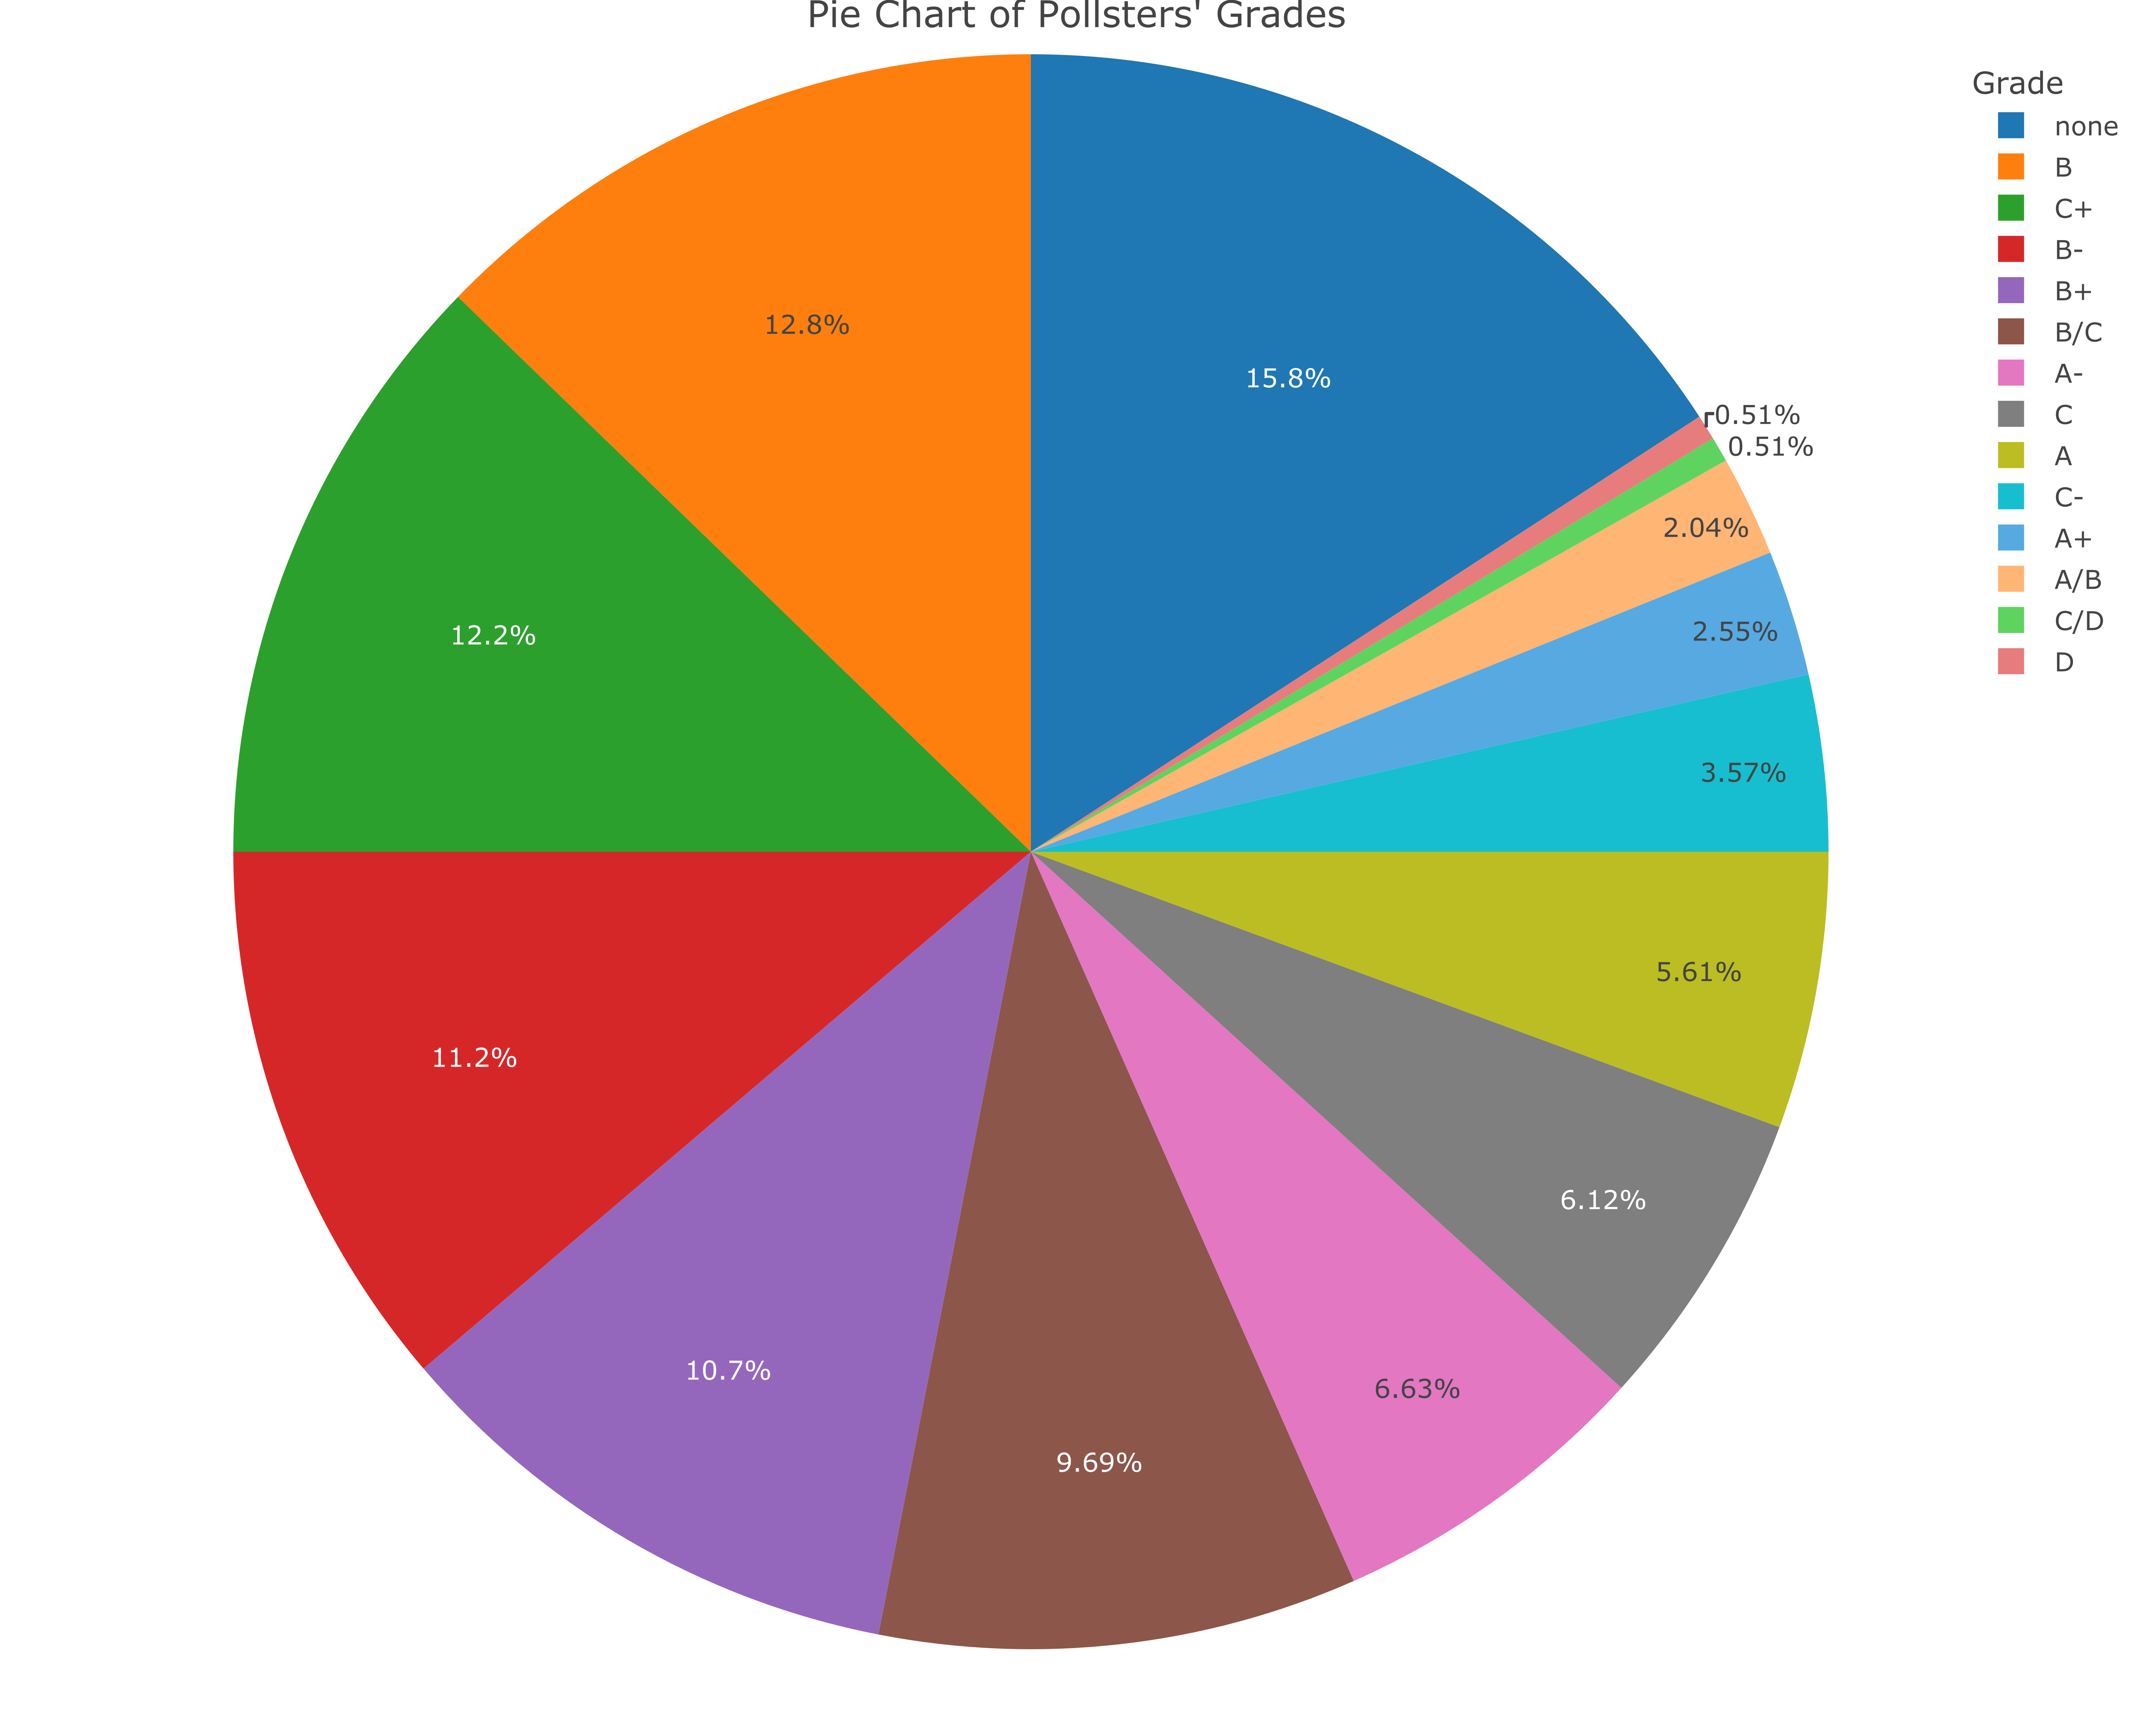
\includegraphics[width=\textwidth,height=0.6\textheight]{./Figures/piechart.png}
\caption{Pollster's Grade Distribution}
\end{figure}

\end{col}

\end{cols}

\hypertarget{sample-size}{%
\subsubsection{Sample Size}\label{sample-size}}

Checking the sample size alone does not inform us much about the poll
result. Instead, we take a look at the distribution of the sample size
with regards to the grade. We sum up the sample size based on each grade
level and made a bar plot:

\begin{minipage}[t]{0.55\textwidth}
\begin{figure}
\includegraphics[width=1\linewidth]{MAT5314-Project-1_files/figure-latex/unnamed-chunk-9-1} \caption{Distribution of Sample Size for Grades}\label{fig:unnamed-chunk-9}
\end{figure}
\end{minipage}
\begin{minipage}[t]{0.45\textwidth}
\vspace{0pt}
As one can see, grade A-, B, C- have the biggest sample size than other grades. The grades were calculated by FiveThirtyEight for each pollster who has its own sample size. Due to the fact that we sum up the sample size, we can conclude that the proportion of the pollsters who receive grade A-, B and C- are greater than those who receive other grades. In addition, we saw that there was a good portion of the sample size that was contributed to the missing grade "none". This portion of the sample therefore does not contribute towards the rating of pollsters. We think that this can reflect the efficiency of the poll. A low portion of the sample size 
\end{minipage}

for the grade ``none'' indicates that the number of pollsters who
gathered those samples and wasn't successfully rated was low. On the
other hand, if the sample size for the grade ``none'' was big, for
example if one had most of the samples with ``none'', then it would mean
that the rating mechanism was not successful or the quality of the poll
was too low to be used for rating pollsters.

\hypertarget{population}{%
\subsubsection{Population}\label{population}}

We now take a look at the population type for which the poll was
sampled. We saw that the population type ``lv'', which stands for likely
voters, count for most of the sample sizes. This is in accordence with
FiveThirtyEight's explanation in their website ``Because the database
covers the final three weeks of the campaign and almost all polling
firms publish likely voter polls by that time, almost all polls in the
database should be likely voter surveys.''.

\begin{figure}
\centering
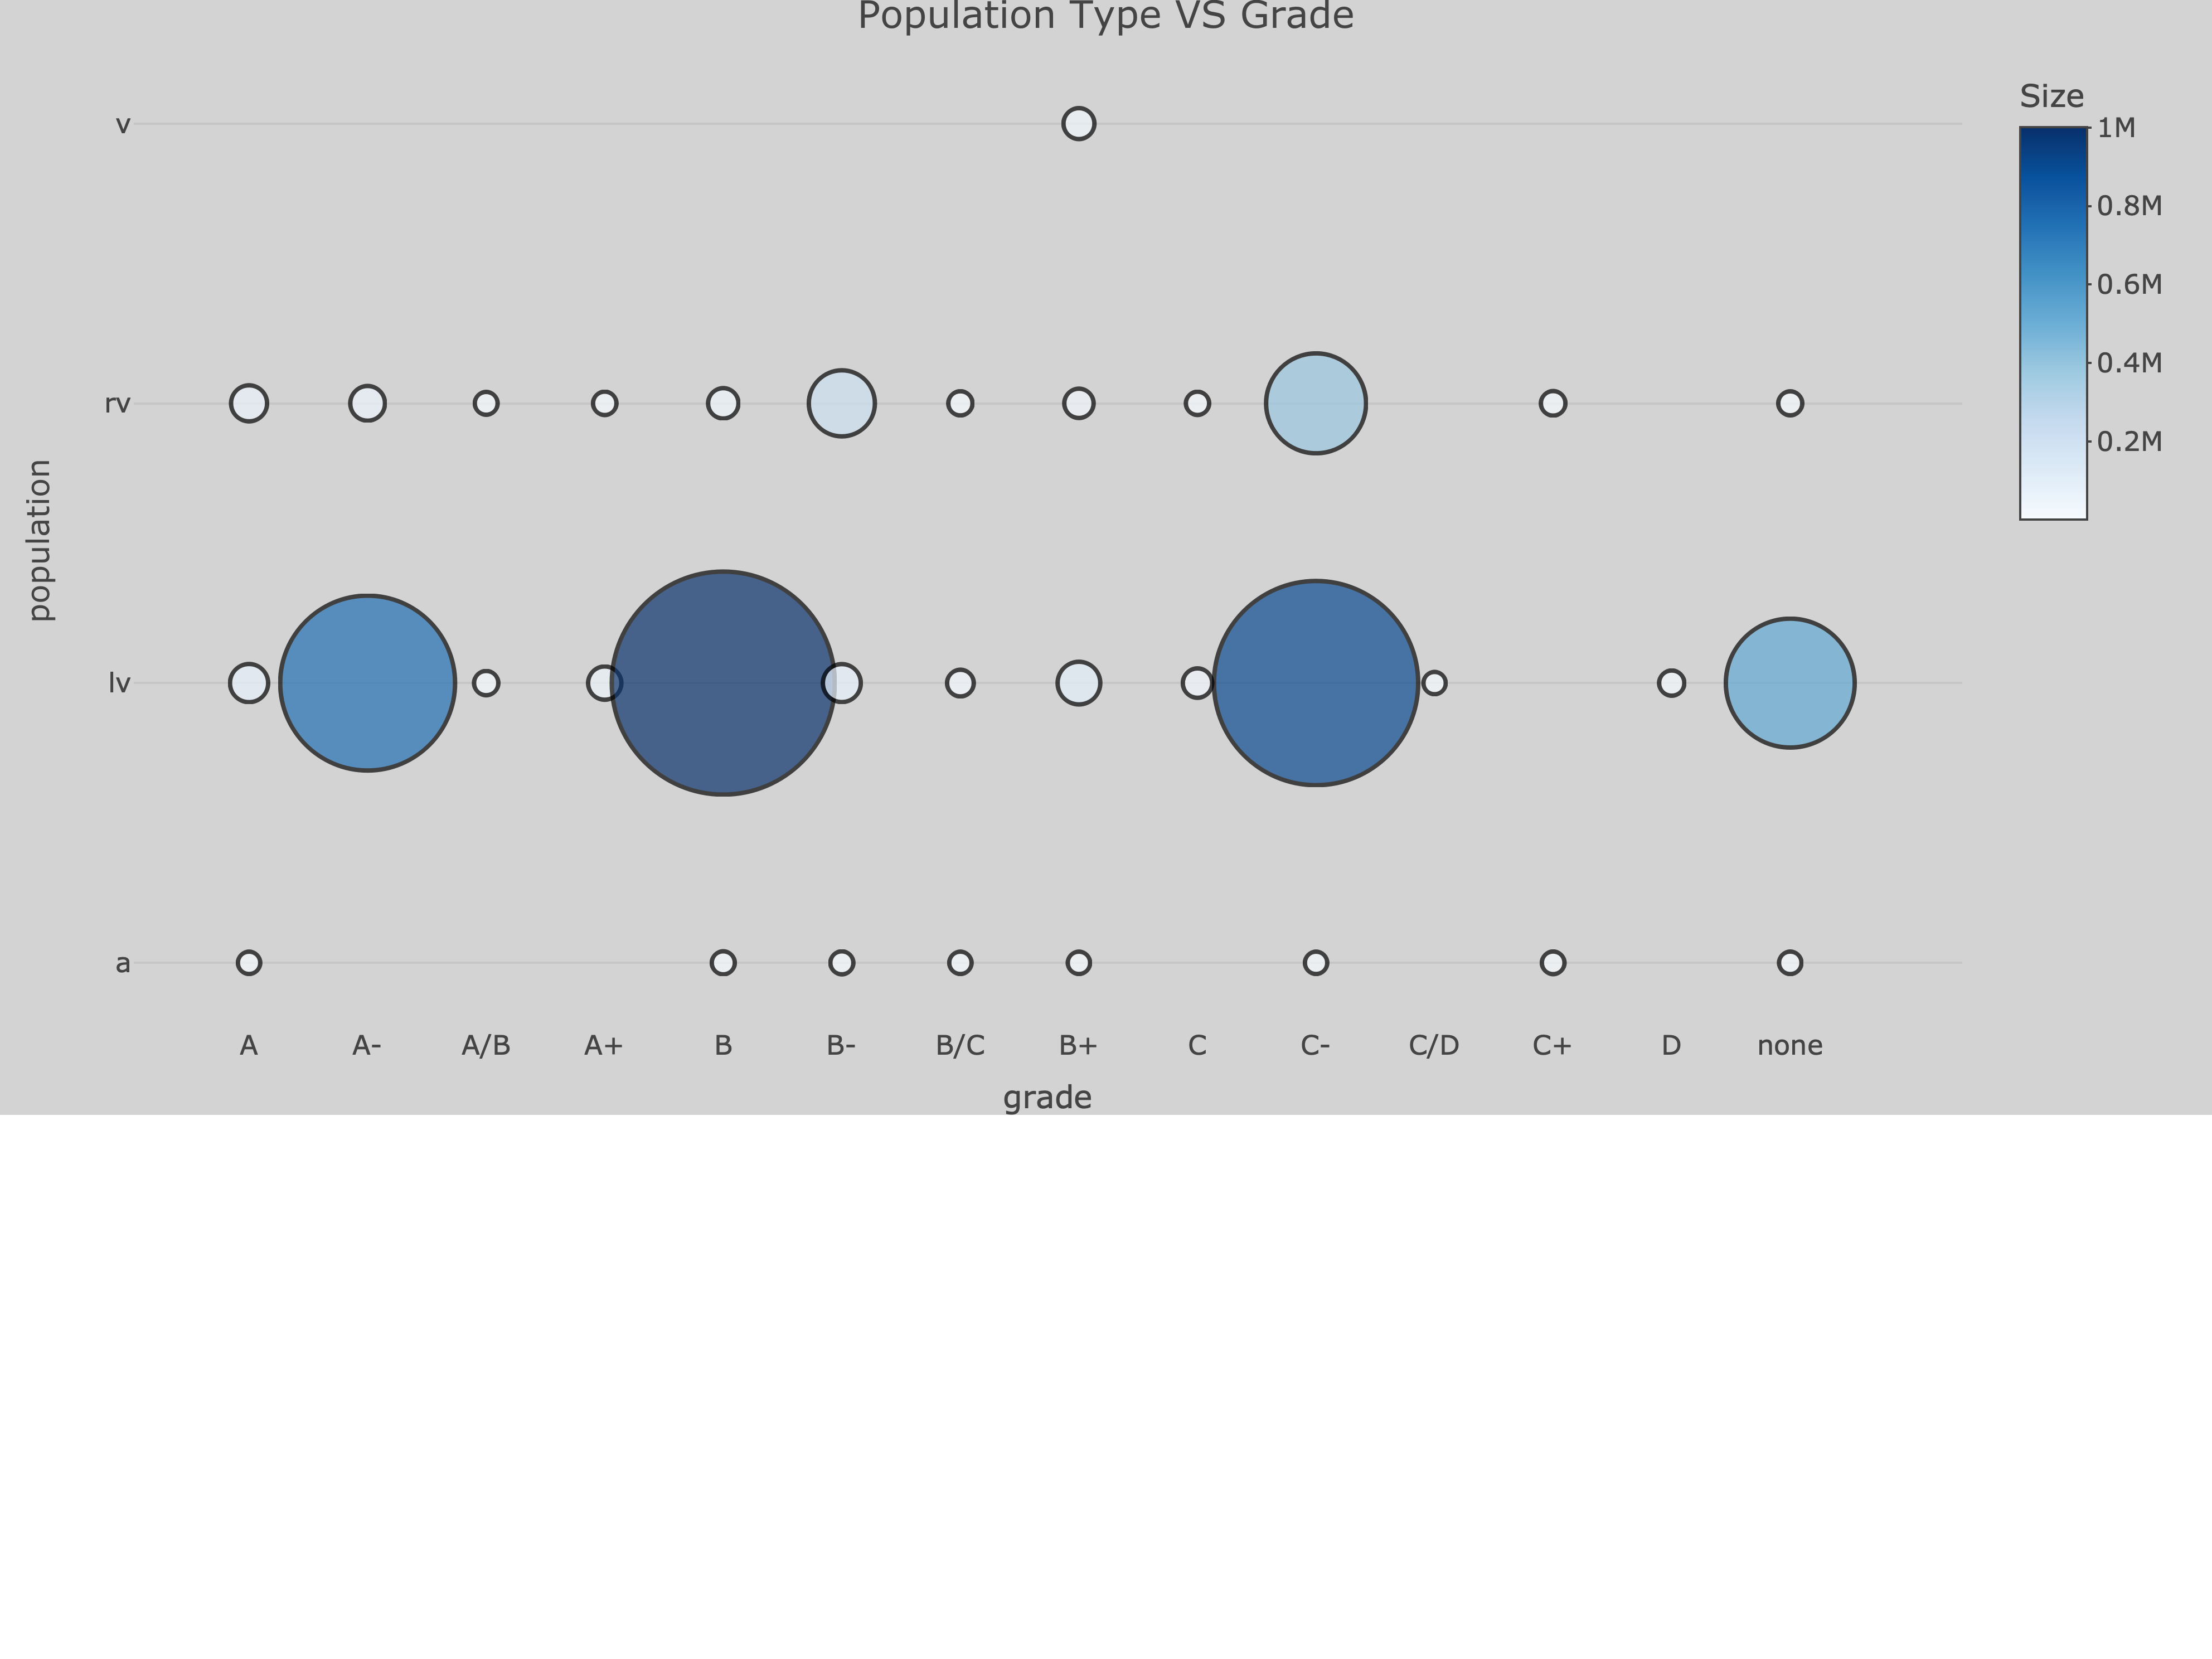
\includegraphics{./Figures/popChart.png}
\caption{Population Type with Size for Grades}
\end{figure}

\hypertarget{poll-rate}{%
\subsubsection{Poll Rate}\label{poll-rate}}

We now turn our attention to the actual poll rate for each candidate.
Using the end date as the standard, we first drew a time series made of
scatter plot of the raw poll rates of the four candidates over time.

\begin{minipage}[t]{0.7\textwidth}
\begin{figure}
\includegraphics[width=1\linewidth]{MAT5314-Project-1_files/figure-latex/unnamed-chunk-12-1} \caption{Raw Poll Proportion by Time}\label{fig:unnamed-chunk-12}
\end{figure}
\end{minipage}
\begin{minipage}[t]{0.3\textwidth}
\vspace{0pt}
Figure 4 indicates that Clinton and Trump’s approval ratings are significantly higher than those of Johnson and Mcmullin at the overall level. Another interesting demonstration is the divergence of support as the vote draws to a close. This shows that as the voting deadline approaches, people's intentions are more inclined to one of Clinton or Trump. Voting is more polarized. A low poll rate for one candidate also implies that other candidates may have high poll rates. This creates differences in each 
\end{minipage}

state. Therefore, we try to compare each candidate's poll result in each
state. We processed the metadata by counting the polls of four
candidates in each state respectively. Result is easy to obtain by
multiplying the given sample size and proportion. Regardless of the
various pollsters, we combine the number of polls for each candidate
received in each state. In this case, we treat NA as 0.

The visualization of the poll proportion of the four candidates in each
state was presented below:

\begin{minipage}[t]{0.7\textwidth}
\begin{figure}
\includegraphics[width=1\linewidth]{MAT5314-Project-1_files/figure-latex/unnamed-chunk-14-1} \caption{Poll Percentage by States}\label{fig:unnamed-chunk-14}
\end{figure}
\end{minipage}
\begin{minipage}[t]{0.3\textwidth}
\vspace{0pt}
Figure 5 shows the poll proportions of the four candidates in each state distinguished by colors. We can clearly observe which candidate is likely to win all the electoral votes in each state, which is helpful in estimating the outcome of the presidential election. From the chart above, we conclude that Clinton and Trump are clearly ahead of Johnson and Mcmullin. 
\end{minipage}

Furthermore, Clinton is clearly ahead of Trump in California, DC,
Hawaii, Illinois, Maryland, Massachusetts, New Jersey, New York, Oregon,
Rhode Island, Vermont, and Washington. Another side, in Alabama, Alaska,
Idaho, Indiana, Iowa, Kansas, Kentucky, Louisiana, Mississippi,
Missouri, Montana, Nebraska, North Dakota, Ohio, Oklahoma, South
Carolina, South Dakota, Tennessee, Texas, Utah, West Virginia, Wyoming,
Trump clearly leads Clinton. This helps us explore the leading
candidates in each state.

We now look at the time series of the adjusted poll proportion:

\begin{minipage}[t]{0.7\textwidth}
\begin{figure}
\includegraphics[width=1\linewidth]{MAT5314-Project-1_files/figure-latex/unnamed-chunk-15-1} \caption{Adjusted Poll Percentage by States}\label{fig:unnamed-chunk-15}
\end{figure}
\end{minipage}
\begin{minipage}[t]{0.3\textwidth}
\vspace{0pt}
We immediately noticed that some of the poll rate for Johnson fell below zero. We did not find a detailed justification to the adjustment they have made from their website, therefore, this makes us to question the validity of the adjusted poll result done by FiveThirtyEight. For other candidates the adjustment was not posing the negativeness issue, so we want to explore if the adjusted data can be ignored or if it actually brings some improvements than the raw poll data.
\end{minipage}

Since the final two candidates in Election 2016 are Clinton and Trump,
we plotted box plots of the difference of their poll results, one for
the raw poll and one for the adjusted poll.

\begin{figure}
\centering
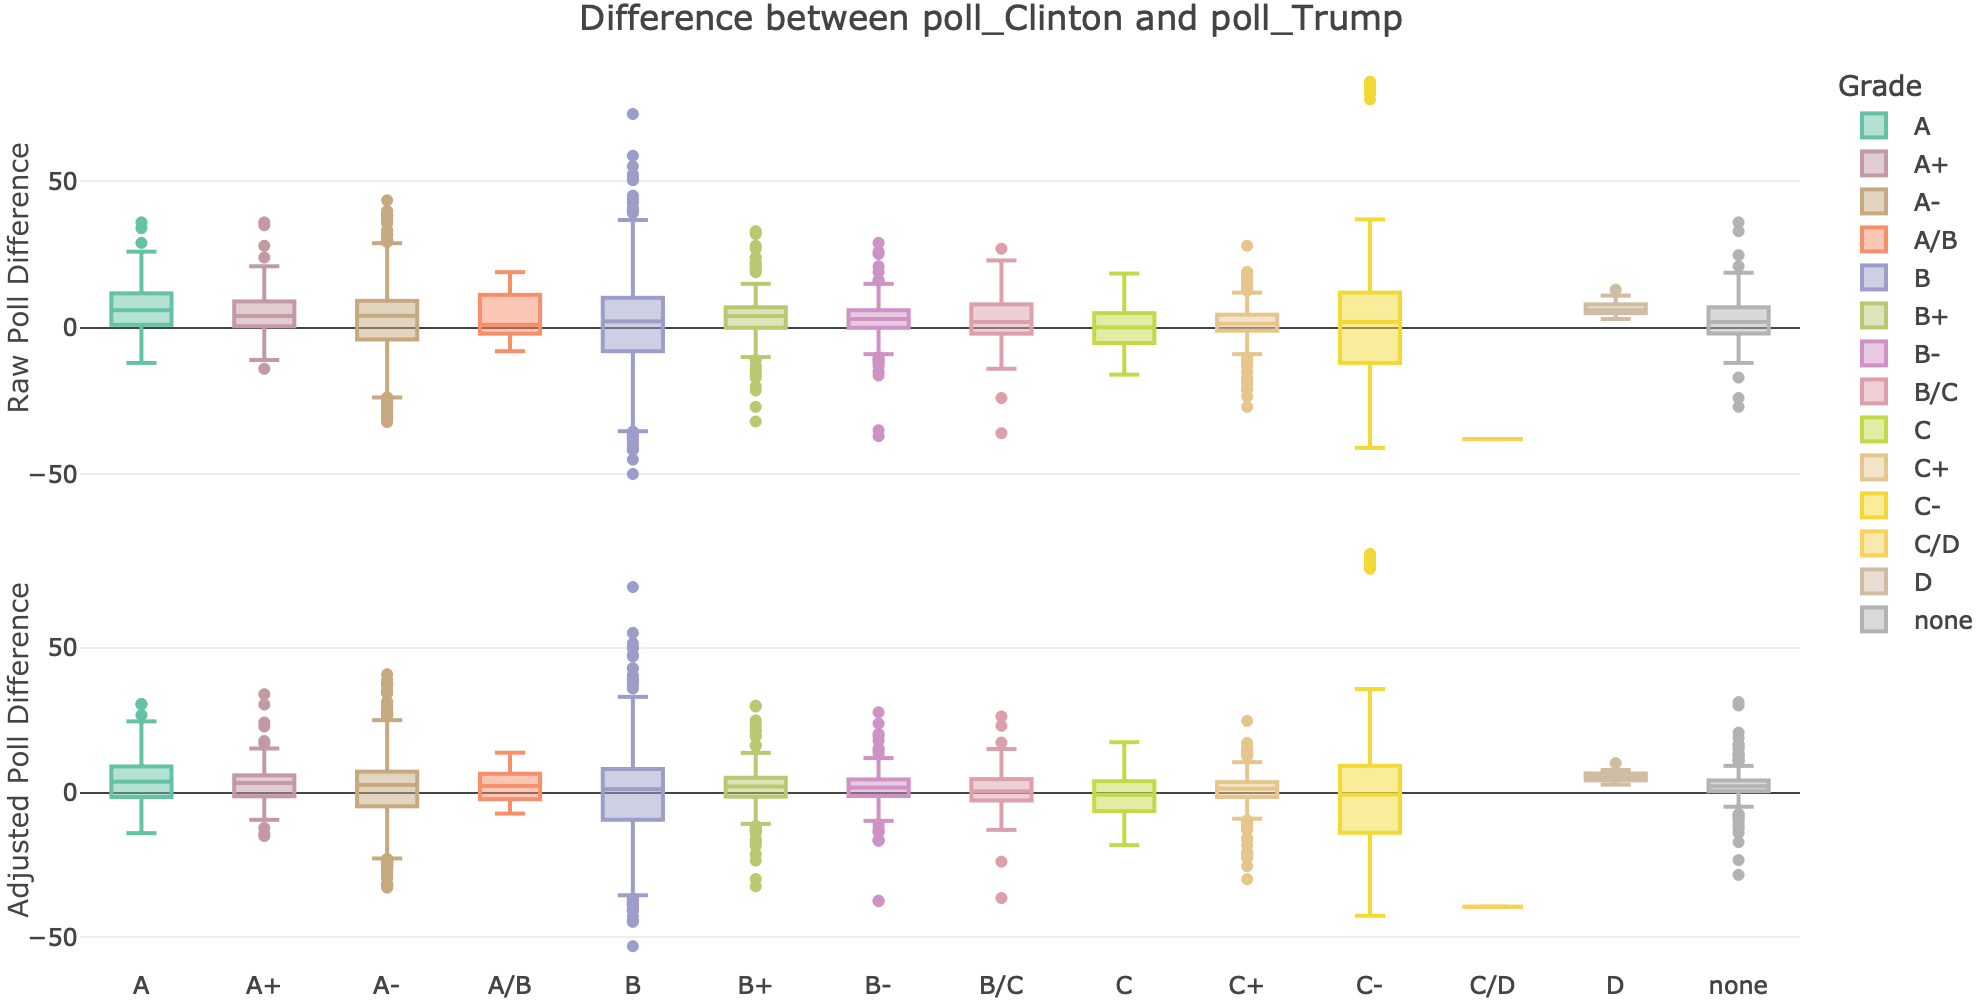
\includegraphics[width=0.7\textwidth,height=\textheight]{./Figures/boxchart.png}
\caption{Boxchart of Difference between Polls}
\end{figure}

We saw that there's little difference between the distribution of the
raw and the adjusted data. However, the mean of each grade of the
adjusted poll result was a little closer to zero than that of the raw
poll result. This indicated that the adjustment that FiveThirtyEight
made was a slight improvement because the raw poll difference of each
grade was mostly above zero, which showed that the poll result was more
in favour of Clinton yet Trump was the final winner of the election.

However, due to the fact that FiveThirtyEight's adjustment to the poll
result yields negative values, we think it is therefore unreasonable to
do such adjustment. It gives the reader a difficulty in interpreting
this adjustment.

Finally we plot the cumulative mean of the raw poll result for the final
two candidates, Trump and Clinton. We selected the Clinton and Trump
polls and ignore the other candidates' poll since the other candidates
are polling far behind Clinton and Trump.

\begin{figure}
\centering
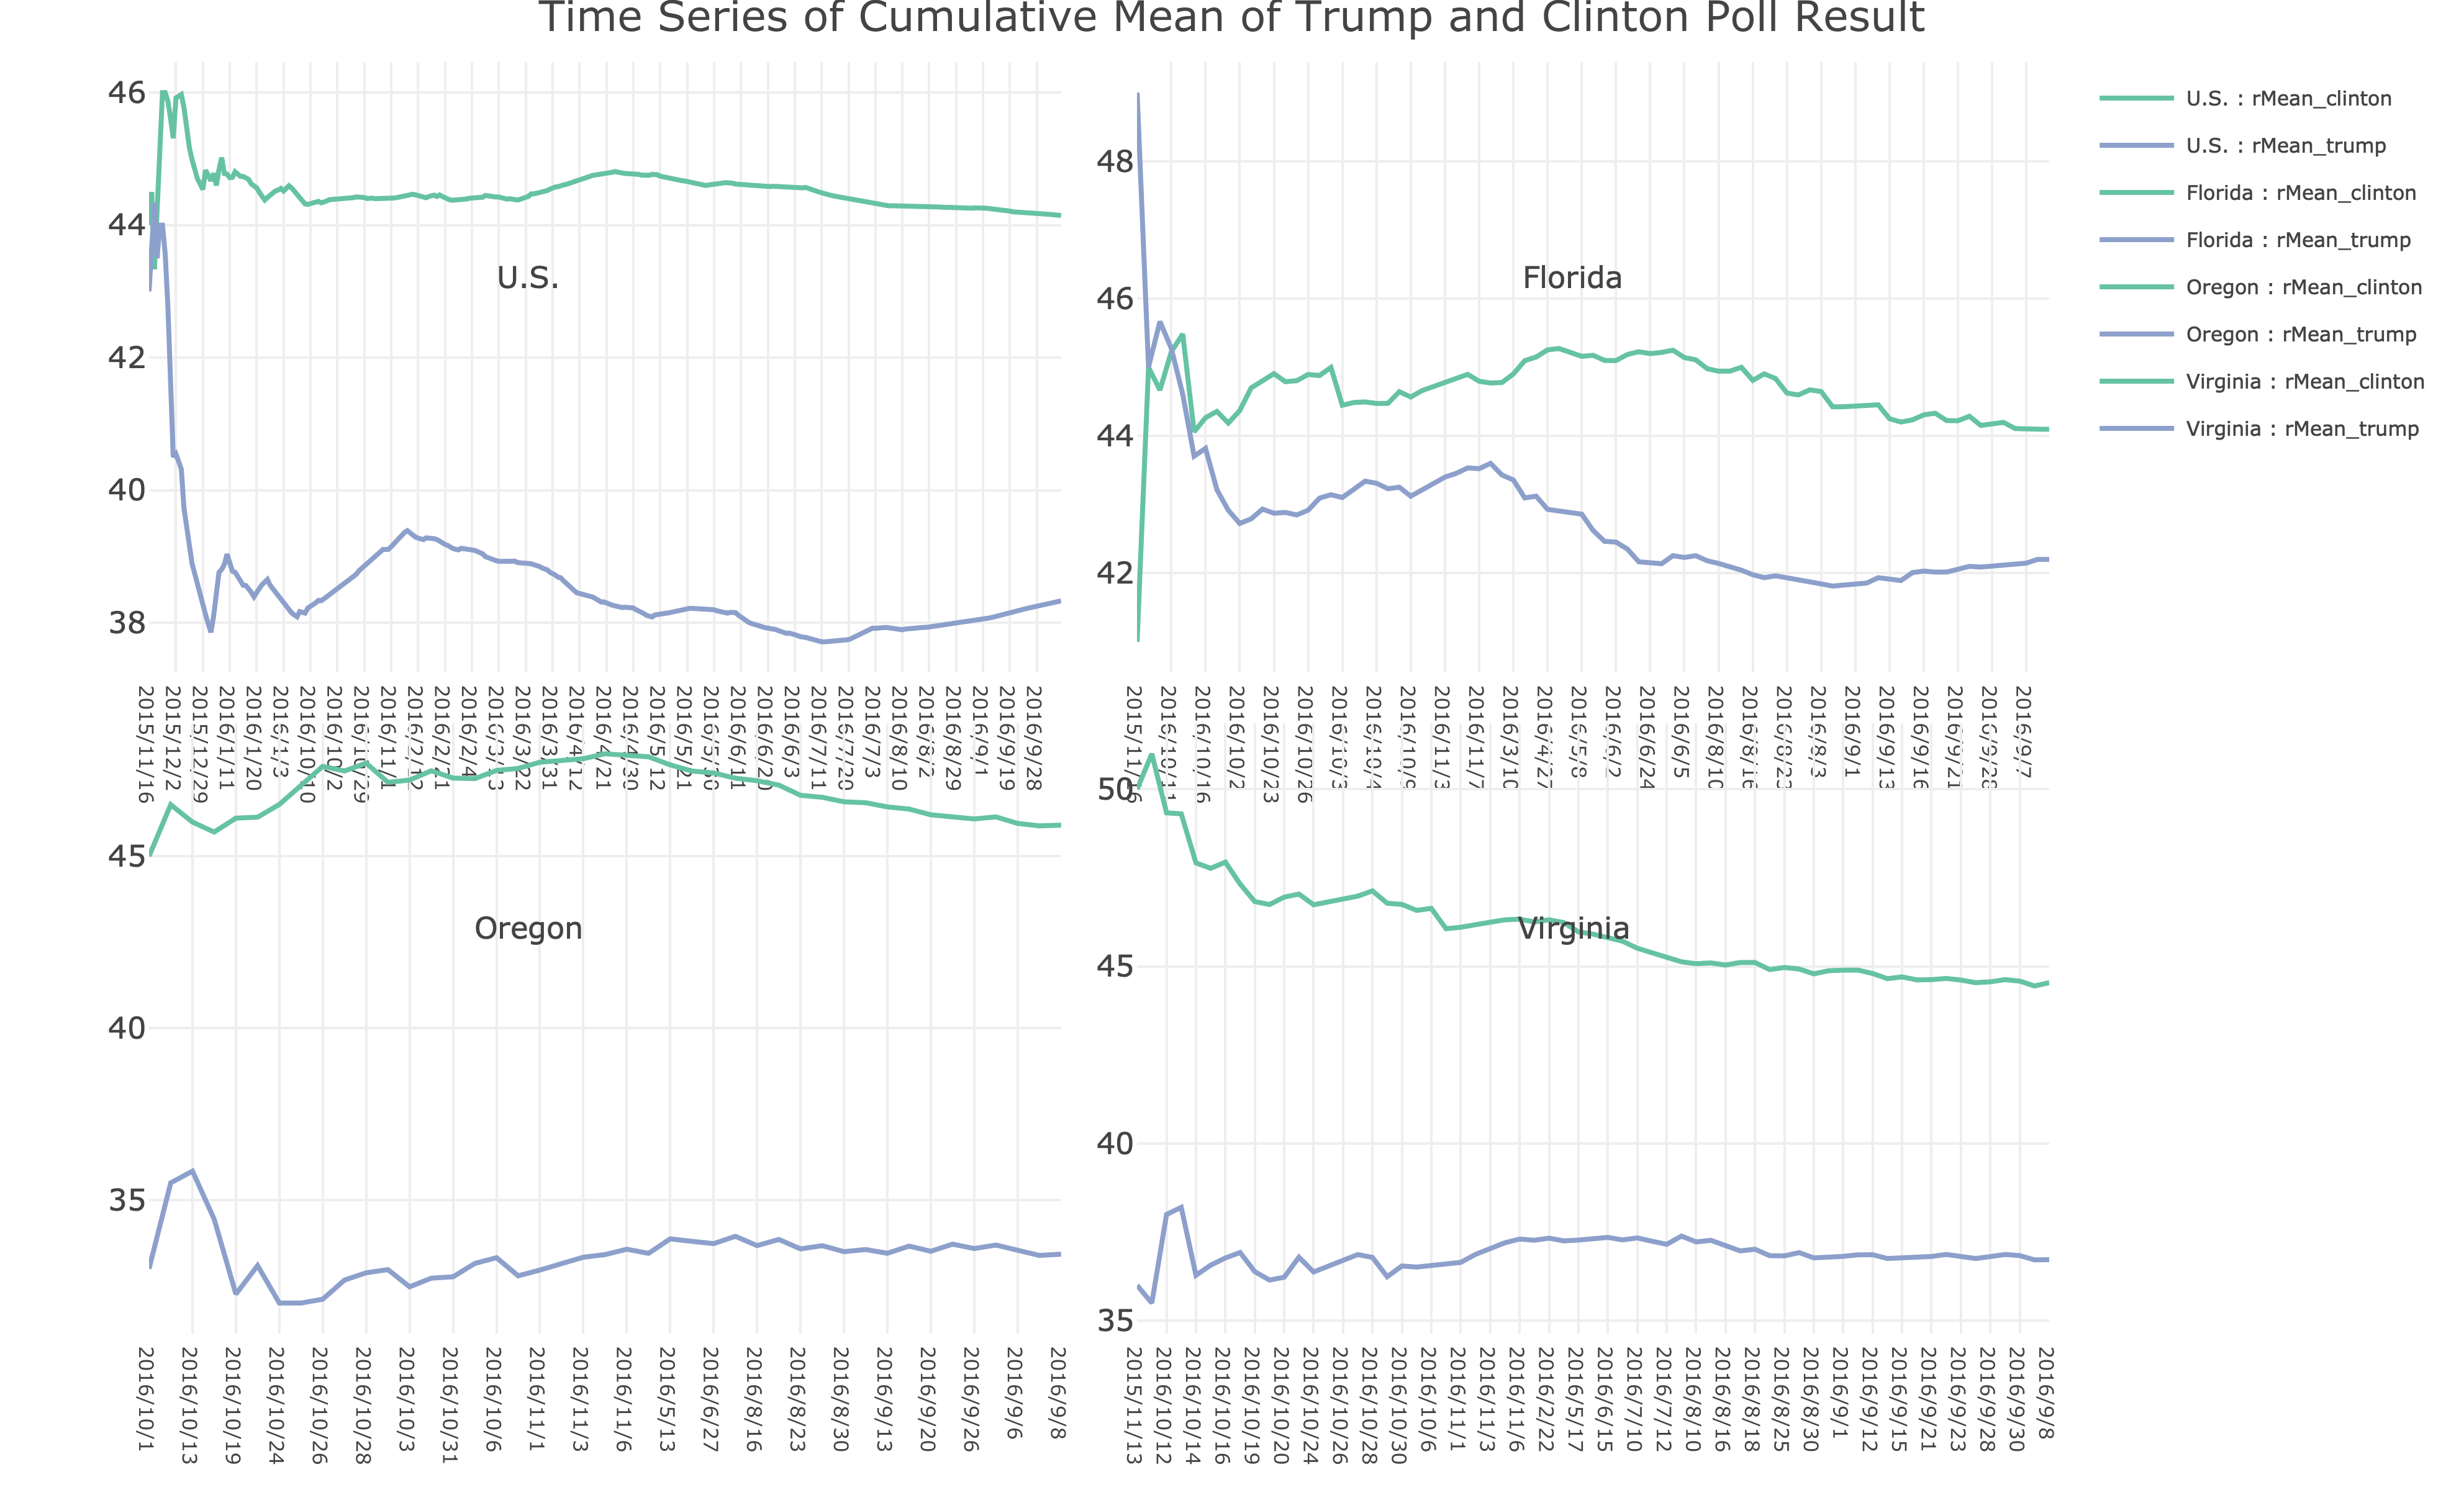
\includegraphics{./Figures/cMeanchart.png}
\caption{Cumulative Mean of Raw Poll Result}
\end{figure}

From the plot above we see that the overall national poll result
indicates that Clinton should be the winner of the election. However,
some of the individual states resulted the opposite conclusion. It it
therefore hard to tell which candidate is leading by examining the
individual state poll result.

\hypertarget{map-chart-of-data}{%
\subsubsection{Map Chart of Data}\label{map-chart-of-data}}

To make state-by-state polling results more visible, we've reflected the
candidates' polling shares on a map of the United States. In the contour
plot below, blue indicates that Clinton is polling proportionally
greater than Trump, and red indicates that Trump is polling
proportionally greater than Clinton. The darker the color, the higher
the proportions are. For states that are nearly white, the margin of
victory is nearly half between Trump and Clinton.

\begin{figure}
\centering
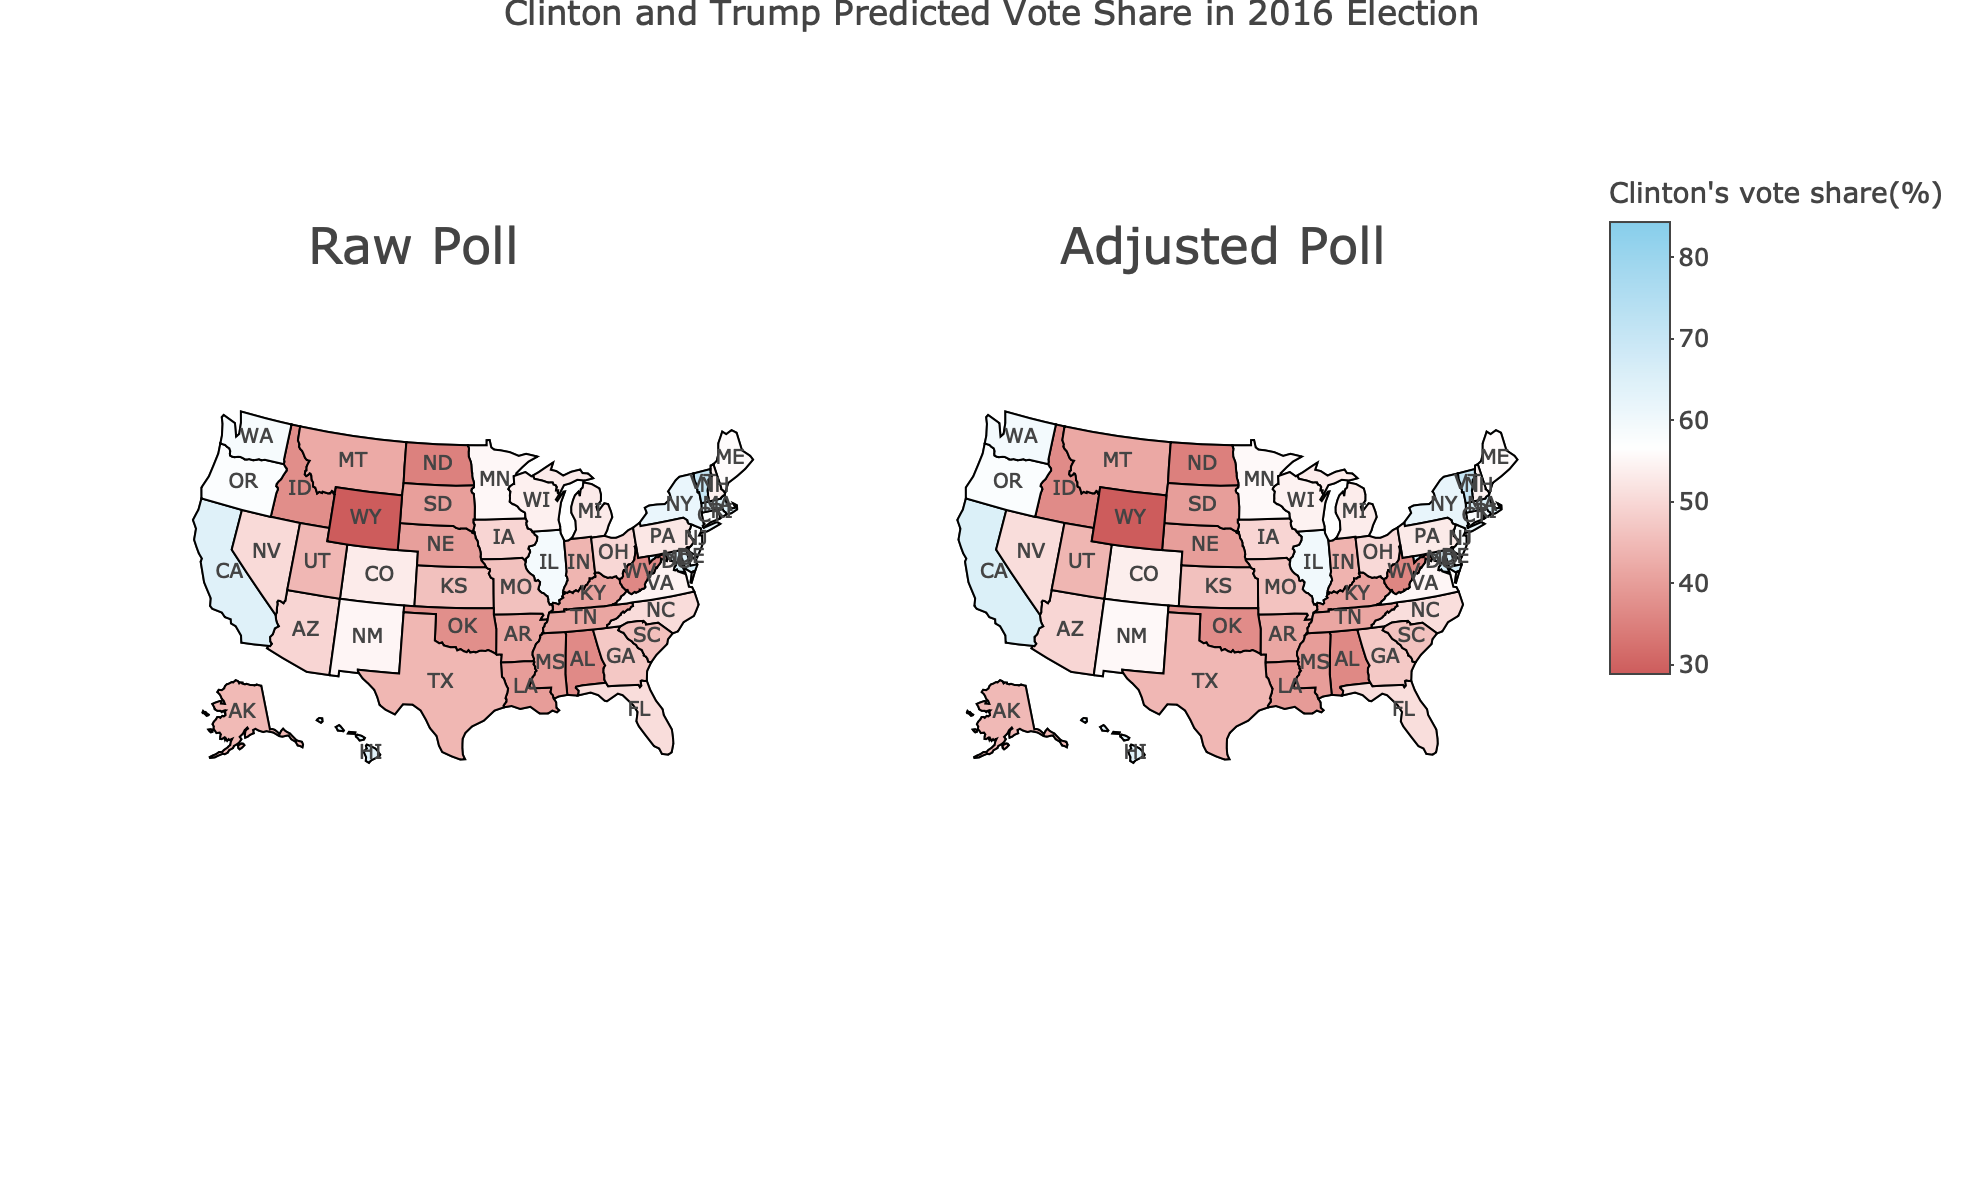
\includegraphics{./Figures/mapchart_1_2.png}
\caption{Map Chart of Vote Shares of Candidates by States}
\end{figure}

We again saw that there was little difference between the results using
the raw poll data and the adjusted poll data, which further support our
opinion that the adjustment made by FiveThirtyEight must be carefully
justified by readers because of its negative values. We then saw from
the map in Figure 9 that Clinton seems to dominate the public opinions
because the colors of states are a bit closer to white and pale red.

Furthermore, we want to find out exactly the states which Clinton or
Trump captured all of the electoral votes. The visualization below shows
the net polls generated by each state for Clinton and Trump.

\begin{minipage}[t]{0.7\textwidth}
\begin{figure}
\includegraphics[width=1\linewidth]{MAT5314-Project-1_files/figure-latex/unnamed-chunk-20-1} \caption{Net Polls by States.}\label{fig:unnamed-chunk-20}
\end{figure}
\end{minipage}
\begin{minipage}[t]{0.3\textwidth}
\vspace{0pt}
Based on raw poll data, Figure 10 shows Clinton won 27 constituencies including 25 states, one additional Maine district and DC. Trump won 25 states plus one additional district in Maine and three additional districts in Nebraska. It is not difficult to see from Figure 10 that Maine and Nebraska have two and three additional electoral district respectively in addition to their own states. The candidate with the most votes in Maine and Nebraska will receive two electoral votes,
\end{minipage}

and the remaining electoral votes will be allocated to the presidential
candidate who wins each district. Moreover, DC have three electoral
votes as an independent district.

Finally, we take a look at the map chart of the electoral votes based on
raw poll result. We use the poll opinion to generate a map showing the
predicted election result, and we compare it with the counterpart
showing the actual final election result.

The Electoral College in the United States consists of 538 electoral
votes. These electoral votes are distributed among the 50 states and the
District of Columbia based on the total number of members in Congress,
which includes both the House of Representatives and the Senate. There
are 435 members in the U.S. House of Representatives. Each state is
given a number of electoral votes equal to its total number of
representatives in the House and it is based on the state's population.
The minimum number of electoral votes a state can have is 3. Then there
are 100 members in the U.S. Senate, with each state having two senators
regardless of its population. Therefore, each state is allocated two
additional electoral votes based on its Senate representation. Finally
we have the District of Columbia. Although the District of Columbia is
not a state, it is granted three electoral votes as if it were a state
of the U.S.. In total, the number of electoral votes is 435 (House of
Representatives) + 100 (Senate) + 3 (District of Columbia) = 538
electoral votes.

To win the U.S. presidential election, a candidate must secure a
majority of these electoral votes, which is currently 270 electoral
votes. This system often leads to a focus on swing states or
battleground states where the outcome is less predictable, as candidates
aim to accumulate enough electoral votes to win the election. In our
Figure 9 map chart, these states tend to have a pale colour due to its
swing opinion.

We obtained the final election result from
(\protect\hyperlink{ref-Final}{2017}).

\begin{figure}
\centering
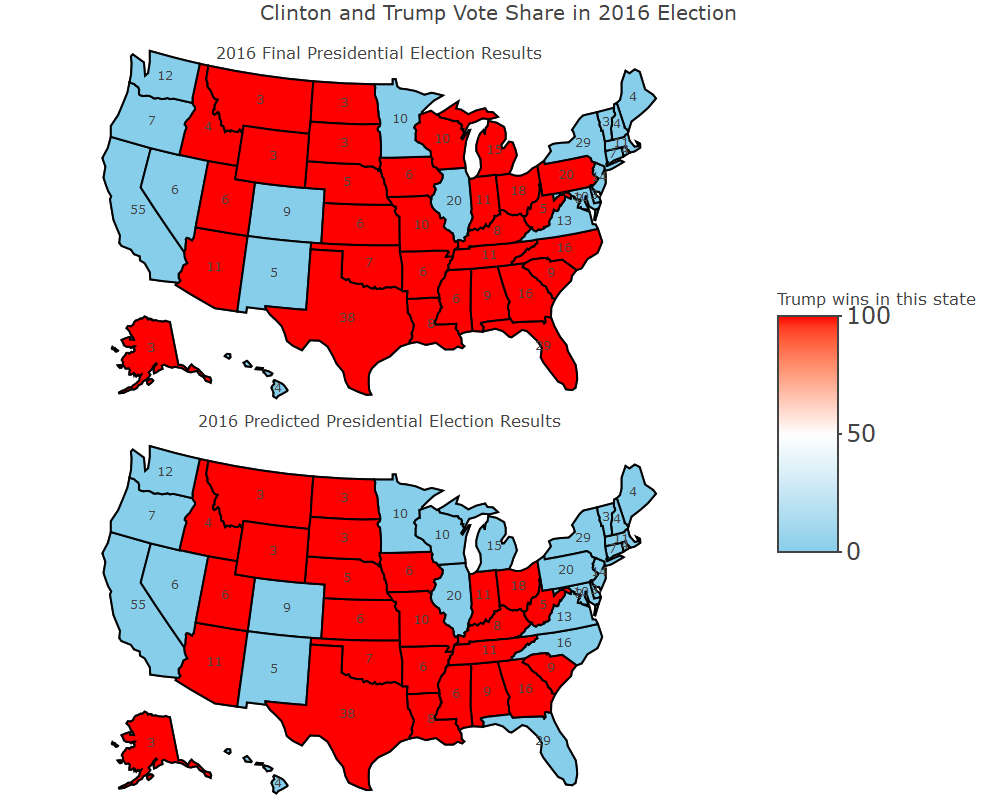
\includegraphics{./Figures/mapchart_3_4.png}
\caption{Map Chart of Election Result 2016}
\end{figure}

From the Figure 11 we can see that the actual final election outcome was
almost the entire opposite to the predicted result. In 2016, Trump won
304 votes compared to 227 votes for Hillary Clinton, which was not
predicted by the election poll result. Therefore, readers must be
careful about the election poll. There have been some criticisms on the
usefulness of these polls (\protect\hyperlink{ref-Critic2}{2022b}). From
the previous analysis in Figure 1, we were also able to find out that
over half of the pollster ratings were between B+ to C and none. This
might suggests that public opinion polls are not as reliable as one
would expect due to the quality of the pollsters.

\hypertarget{conclusion}{%
\section{Conclusion}\label{conclusion}}

\hypertarget{references}{%
\section*{References}\label{references}}
\addcontentsline{toc}{section}{References}

\hypertarget{refs}{}
\begin{CSLReferences}{1}{0}
\leavevmode\vadjust pre{\hypertarget{ref-Final}{}}%
2017. \url{https://www.nytimes.com/elections/2016/results/president}.

\leavevmode\vadjust pre{\hypertarget{ref-Critic2}{}}%
---------. 2022b.
\url{https://thehill.com/homenews/campaign/3718434-optimistic-democrats-insist-the-polls-are-wrong/}.

\leavevmode\vadjust pre{\hypertarget{ref-Critic}{}}%
---------. 2022a.
\url{https://gelliottmorris.substack.com/p/the-polling-website-where-republicans}.

\leavevmode\vadjust pre{\hypertarget{ref-MissingD}{}}%
---------. 2023.
\url{https://projects.fivethirtyeight.com/pollster-ratings/}.

\end{CSLReferences}

\end{document}
